
\documentclass{beamer}
\usepackage[orientation=portrait, size=a1, scale=1.4, debug]{beamerposter}
\usetheme{unn}

\usepackage{cmbright}

\usepackage{fontspec}

\setmainfont{Times New Roman}
\setromanfont{Times New Roman}
\setsansfont{Times New Roman}

\usepackage{polyglossia}
\setmainlanguage{russian}
\usepackage{csquotes}

\usepackage{booktabs}
\usepackage{ragged2e}

\usepackage[backend=biber,
            movenames=false,
            maxnames=4,
            style=gost-numeric,
            sorting=nty,
            autolang=other]{biblatex}
						
%\newfontfamily\cyrillicfonttt{lmmonolt10-regular.otf}
%\newfontfamily\cyrillicfontsf{lmsans10-regular.otf}						
					
\addbibresource{bibliography.bib}

\DeclareMathOperator{\re}{\operatorname{Re}}

\title{Решение многомерных задач глобальной оптимизации с использованием Intel oneAPI }
\author{К.А. Баркалов \and И.Г. Лебедев \and Я.В. Кольтюшкина}
\institute{Нижегородский государственный университет им. Н.И. Лобачевского}
\setlength{\abovedisplayskip}{3pt}
\setlength{\belowdisplayskip}{3pt}

\begin{document}
\begin{frame}[t]
    \begin{columns}[t]
        \begin{column}[t]{0.47\paperwidth}
            \begin{block}{Постановка задачи}
             Задача многомерной многоэкстремальной оптимизации может быть определена как поиск наименьшего значения действительной функции \(\phi(y)\)  в гиперинтервале \(D=\{y\in R^N:a_i\leqslant x_i\leqslant{b_i}, 1\leqslant{i}\leqslant{N}\}\). 
             
             Будем предполагать, что целевая функция задана по принципу <<черного ящика>> и удовлетворяет условию Липшица с априори неизвестной константой \(L\). 

          \end{block}
          
          \begin{block}{Редукция размерности с помощью кривых Пеано}

В ННГУ им. Н.И. Лобачевского под руководством проф. Р.Г. Стронгина разработан эффективный подход к решению задач глобальной оптимизации \cite{Strongin2013}. В рамках данного подхода решение многомерной задачи сводится к решению эквивалентной ей одномерной задачи. Для этого используется редукция размерности с помощью кривой Пеано \(y(x)\), которая непрерывно и однозначно отображает отрезок вещественной оси \([0,1]\) на \(N\)-мерный куб \cite{Sergeyev2013}.

 \begin{minipage}[t]{.47\textwidth}
              \begin{figure}
                  \centering
                  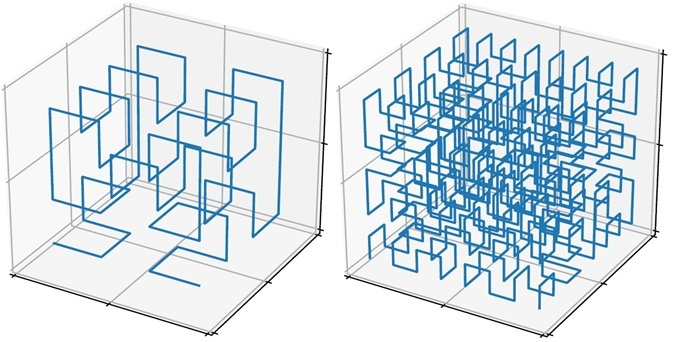
\includegraphics[scale=1.49]{images/pean_2.jpg}
              \end{figure}
              \end{minipage}
              


\end{block}
\begin{block}{Метод глобальной оптимизации}

В процессе работы алгоритма строится последовательность точек \(x^k\), в которых проводятся \textit{испытания}, т.е. вычисляются значения целевой функции \(\phi^k=\phi(y(x^k))\). 

Распараллеливание организовано следующим образом: в ходе выполнения одной итерации алгоритма одновременно проводятся \(P \geq 1\) испытаний в наиболее перспективных точках области поиска. В прикладных задачах глобальной оптимизации проведение даже одного испытания является трудоемкой операцией. Поэтому параллельное проведение нескольких испытаний повышает скорость работы алгоритма. 

 \begin{minipage}[t]{.47\textwidth}
              \begin{figure}
                  \centering
                  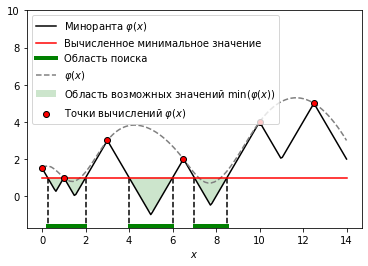
\includegraphics[scale=2.05]{images/PlotGS_1.png}
              \end{figure}
              \end{minipage}
\end{block}
            
        \end{column}
        \begin{column}[t]{0.47\paperwidth}
          \begin{block}{Общая схема параллельного алгоритма}

Одна итерация состоит в выполнении следующих действий:
              \begin{enumerate}
                \justifying
                \item Упорядочить точки предшествующих испытаний в порядке возрастания их координат: \(x_{0}<...<x_{i}<...<x_{k}\);
                \item Для каждого интервала \((x_{i-1}, x_{i}),1\leqslant i\leqslant k,\) вычислить его \textit{характеристику} \(R(i)\);
                \item Упорядочить характеристики \(R(i)\) в порядке убывания \(R(t_{1})\geqslant R(t_{2})\geqslant ... \geqslant  R(t_{k-1})\geqslant R(t_{k})\) и выбрать \(P\) интервалов \((x_{t_j-1}, x_{t_j}), 1\leqslant j \leqslant P,\) с наибольшими характеристиками;
                \item Провести следующие испытания параллельно в точках  \(x^{k+j} \in (x_{t_j-1}, x_{t_j})\), \(1\leqslant j \leqslant P,\) вычисляемых согласно правилу размещения точки следующего испытания в интервале с заданным номером \(t_j\);
                \item Проверить выполнение критерия остановки \(\Delta_{t_j}<\varepsilon, 1\leqslant j \leqslant P\).
              \end{enumerate}

\end{block}

\begin{block}{Использование Intel oneAPI}

Мы реализовали рассмотренный параллельный алгоритм с использованием набора инструментов Intel oneAPI. Достоинством Intel oneAPI является простота, открытость и возможность легкой интеграции в существующий код. Intel oneAPI позволяет написать код один раз и в дальнейшем запускать его на различных устройствах. 

При реализации мы использовали возможности распараллеливания, которые обеспечиваются языком Data Parallel C++ и набором библиотек Intel oneAPI, облегчающих межархитектурную разработку.   


\end{block}
%----------------------------------------------------------------------------------------
%	RESULTS
%----------------------------------------------------------------------------------------

\begin{block}{Результаты}

На данный момент получены результаты вычислительных экспериментов на тестовых задачах, формируемых специальным генератором \cite{GKLS}. В таблицах \ref{table:GKLS_RES_1}, \ref{table:GKLS_RES_2} приведены среднее число итераций параллельного алгоритма глобального поиска и ускорение относительно последовательной версии. В каждом эксперименте решалось 100 задач размерности \(N = 4\) и \(N = 5\). Эксперименты проведены на компьютере с процессором Intel Core I5-7300HQ 2.5 GHz с видеокартой HD Graphics 630, 16 GB RAM, использовался язык \textit{Data Parallel C++}.


%{\setlength{\extrarowheight}{5pt}

\begin{table}[!hbp]
    \centering
    \caption{Число итераций и ускорение при решении серии задач размерности $N=4$}
     \renewcommand{\arraystretch}{1.4}
    \renewcommand{\tabcolsep}{1cm}
    \begin{tabular}{|c|c|c|c|}
    \hline
    P  & Итерации  & Время работы (сек.) & Ускорение \\ \hline
	128 & 106.5 & 1.2  & 4.7    \\ \hline
	256 & 41.3 & 0.66   & 8.5          \\ \hline
	\end{tabular}
    
    \label{table:GKLS_RES_1}
\end{table}

\begin{table}[!hbp]
    \centering
    \caption{Число итераций и ускорение при решении серии задач размерности $N=5$}
    \renewcommand{\arraystretch}{1.4}
    \renewcommand{\tabcolsep}{1cm}
    \begin{tabular}{|c|c|c|c|}
    \hline
    P  & Итерации  & Время работы (сек.) & Ускорение \\ \hline
	128 &        235.6 & 2.6  & 4.4      \\ \hline
	256 &       90.5  & 1.2 & 9.2      \\ \hline
	\end{tabular}
    
    \label{table:GKLS_RES_2}
\end{table}

\end{block}
          \begin{block}{Литература}
            \printbibliography
            
          \end{block}
        \end{column}
    \end{columns}
\end{frame}
\end{document}
